\documentclass{article}
\usepackage{amsmath}
\usepackage{amssymb}
\usepackage{graphicx}
\usepackage{hyperref}
\usepackage[version=4]{mhchem}

\title{Problem 12}
\date{}

\begin{document}
\maketitle

\section*{Problem}
As shown in the figure, two diagonals \(A C\) and \(B D\) of quadrilateral \(A B C D\) intersect at \(O\). Find the length of \(A D\) if \(B O=6, O D=\) \(14, A O=15, O C=7\), and \(A B=10\).\\
(A) \(9 \sqrt{7}\)\\
(B) \(8 \sqrt{7}\)\\
(C) \(6 \sqrt{7}\)\\
(D) \(8 \sqrt{2}\)\\
(E) \(10 \sqrt{7}\)\\
\centering
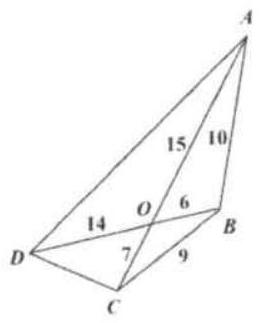
\includegraphics[width=\textwidth]{images/090(2).jpg}

\section*{Solution}
Solution not available.

\end{document}
